\chapter{系统分析与设计}

\section{需求分析}

本视频编辑系统的需求分析基于技术可行性研究,主要涵盖功能性需求、非功能性需求、技术约束和用户场景等方面。

在功能性需求方面,首先,多模态视频编辑功能应支持文本指令驱动、
参考图像风格迁移、虚拟换装和光照调整等多种编辑方式。其次,考虑到编辑过程需要预处理以及多轮训练,
系统无法实时的生成结果,因此需要在结果生成后告知用户。最后,作为实验室算法的展示平台,系统需要
具备一定的扩展性,以便于后续的算法更新和功能扩展。

非功能性需求方面,系统需要具备较高的安全性,应当采取的措施包括用户认证、数据库信息加密、前后端分离、
API接口鉴权等。此外,系统应该具有较好的可维护性,包括代码规范、模块化设计、应用文档编写等,以方便后续的维护和升级。

技术约束方面,系统部署在实验室服务器上,配置了cuda12.1与小规模计算平台,运算资源有限;同时由于部署在学校内网无法
直接通过外网访问,需要网络地址转换(NAT)技术提供访问支持。

用户场景方面,一方面该系统面向对最新人工智能技术感兴趣的研究者及普通用户,需要提供简洁易用的界面和友好的交互体验;
另方面该系统面向实验室研究者,为他们提供了解用户真实需求的渠道,需要提供相关的数据统计和分析功能。

\section{概要设计}

系统概要设计的主要任务是将一个复杂的系统按功能划分成模块,确定每个模块的功能及模块之间的调用关系;确定模块之间的
接口,即模块之间的数据传递方式。另外,根据系统涉及到的实体与实体间的关系,设计数据库的表结构。

\subsection{架构设计}

我们采用分层微服务架构,结合事件驱动的设计模式,将系统划分为客户端层、服务层、数据层,如~\ref{fig:system_structure}所示。
客户端层提供响应式用户界面,并处理用户交互事件;服务层由Flask微服务集群组成,负责处理客户端请求,
并与数据层通信进行数据存储和检索;数据层使用MySQL数据库存储用户信息、任务信息和编辑结果,使用Redis数据库存储任务队列和任务状态。

\begin{figure}[ht]
    \centering
    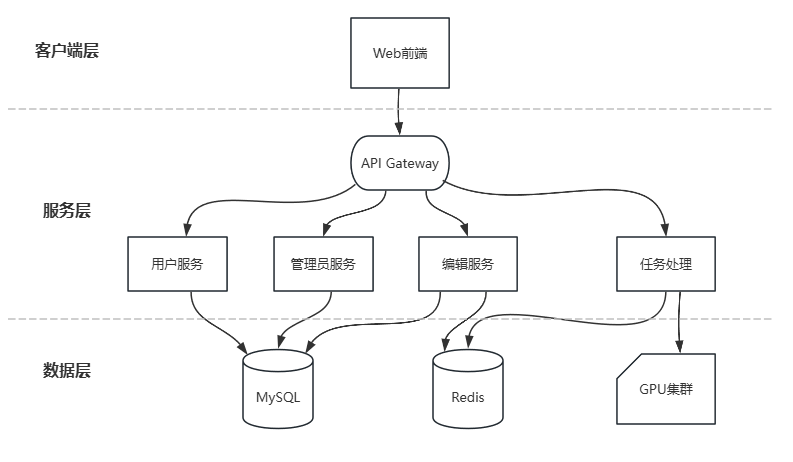
\includegraphics[width=0.6\textwidth]{source/img/system_structure.png}
    \bicaption{系统架构图}{System Architecture Diagram}
    \label{fig:system_structure}
\end{figure}

\subsection{数据库设计}

根据需求分析,我们设计了用户表、任务表和编辑结果表,如~\ref{fig:database_design}所示。考虑到文件管理的需要,
我们在文件相关的表中添加了过期时间字段,以方便后续的文件清理工作。

\begin{figure}[ht]
    \centering
    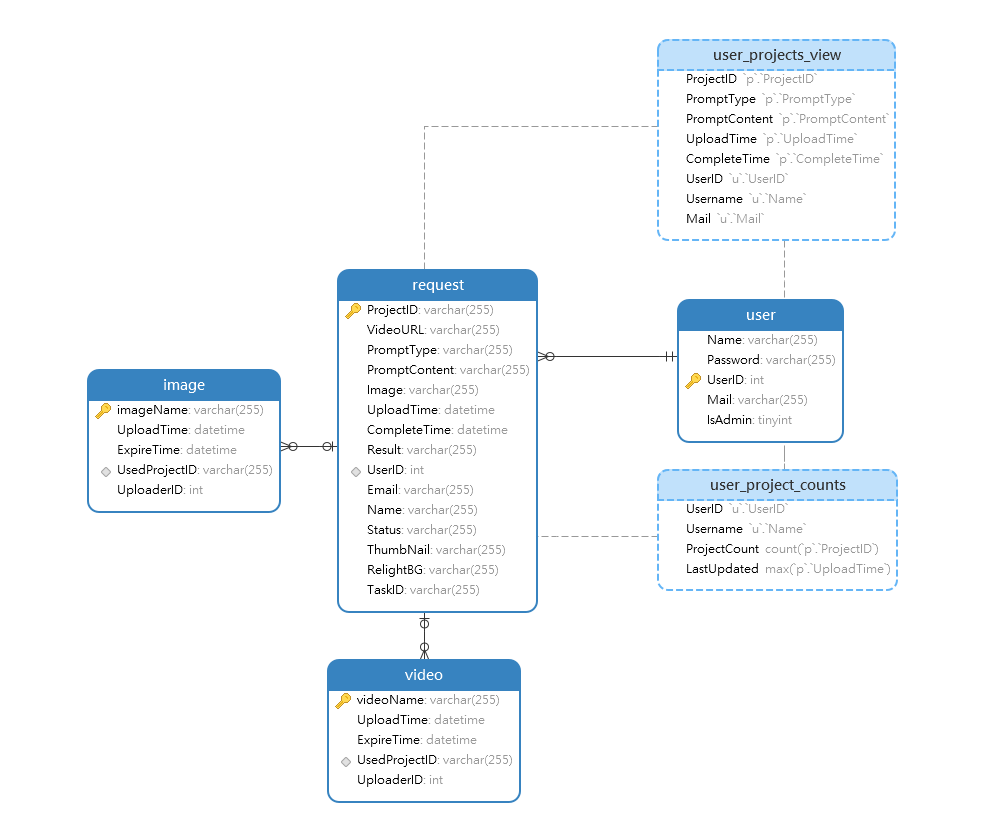
\includegraphics[width=0.6\textwidth]{source/img/database_design.png}
    \bicaption{数据库ER图}{Database ER Diagram}
    \label{fig:database_design}
\end{figure}

\section{详细设计}

\subsection{用例设计}

一般用户在登录后可以上传视频并进行编辑、查询与管理编辑结果,并且可以查看开发者的相关信息。用户用例图如~\ref{fig:user_uml}所示。
\begin{figure}[ht]
    \centering
    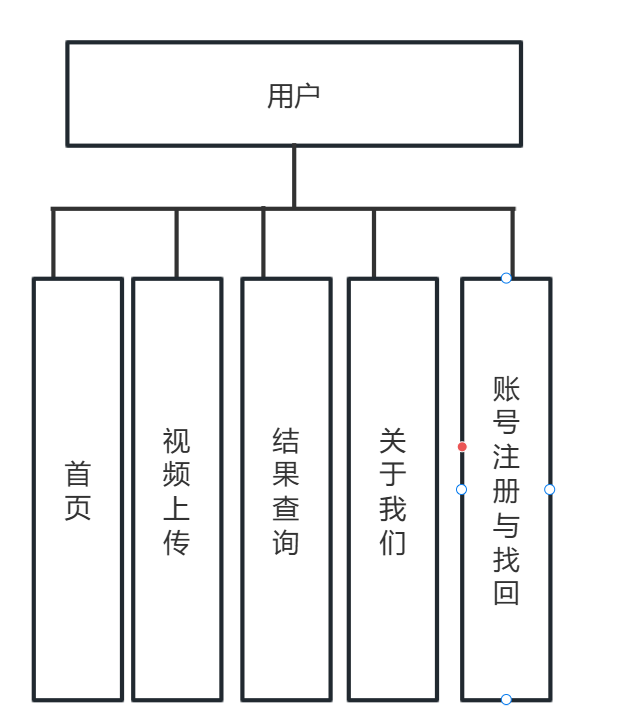
\includegraphics[width=0.3\textwidth]{source/img/user_uml.png}
    \bicaption{用户用例图}{User Use Case Diagram}
    \label{fig:user_uml}
\end{figure}
管理员用户除了一般用户所拥有的功能之外,还添加了数据统计与任务请求导出功能,以方便实验室研究者了解用户真实需求。管理员用户用例图如\ref{fig:admin_uml}所示。
\begin{figure}[ht]
    \centering
    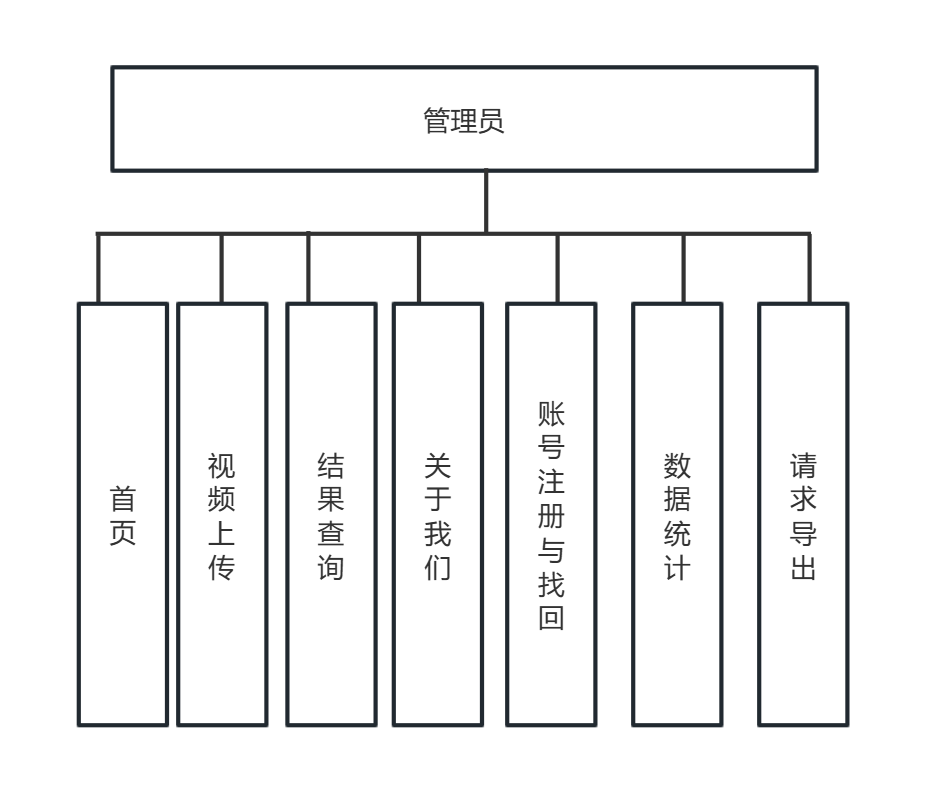
\includegraphics[width=0.4\textwidth]{source/img/admin_uml.png}
    \bicaption{管理员用例图}{Admin Use Case Diagram}
    \label{fig:admin_uml}
\end{figure}

\subsection{流程设计}

系统涉及到的工作流程主要包括登陆管理、任务上传与结果管理。

\subsubsection{登录管理}

由于用户的编辑结果通过邮箱来发送,我们可以将邮箱作为用户的唯一标识,在用户注册时将邮箱作为用户名,密码作为用户密码,通过邮箱和密码进行登录。
用户忘记密码时也可以通过邮箱进行密码重置。登录流程如\ref{fig:login_process}所示。
\begin{figure}[ht]
    \centering
    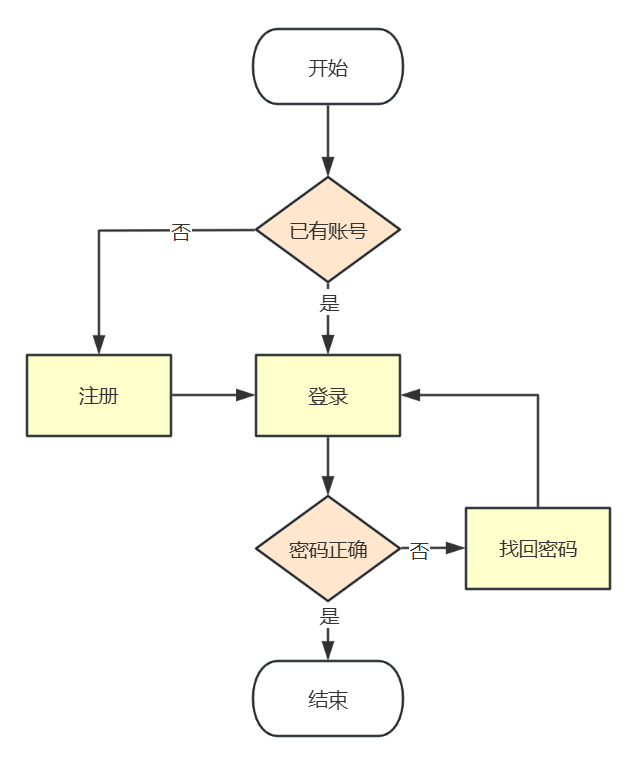
\includegraphics[width=0.4\textwidth]{source/img/login_process.png}
    \bicaption{登录流程图}{Login Process}
    \label{fig:login_process}
\end{figure}

\subsubsection{任务上传}

根据视频编辑算法的输入,需要用户提供视频、编辑提示类型与对应的提示内容,并提供邮箱以获取编辑结果。上传流程如\ref{fig:upload_process}所示。
\begin{figure}[ht]
    \centering
    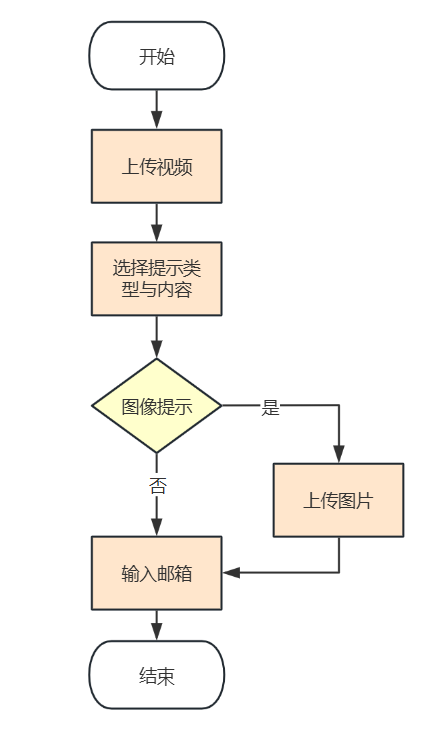
\includegraphics[width=0.3\textwidth]{source/img/edit_process.png}
    \bicaption{上传流程图}{Upload Process}
    \label{fig:upload_process}
\end{figure}

\subsubsection{结果管理}

用户在结果查询界面可以查看自己上传的任务进度与结果,系统也支持任务重命名与删除,同时在任务处理完成后会自动生成略缩图,方便用户预览结果。

\subsection{安全控制设计}

在系统构建的过程中,安全控制是一个至关重要的方面。为了防止未经授权的访问和操作,我们需要用户在登录状态下进行操作,这涉及到对用户信息与数据的
加密保护;我们也需要限制用户的操作行为,以防止用户的恶意操作;另外为了保证服务器的安全性,我们也需要系统部署过程中的安全措施。

\subsubsection{用户信息与数据加密}

我们将用户信息存储在数据库中,包括用户名、密码、邮箱等敏感信息。为了保证用户信息的安全性,我们对输入信息加密后存储。
我们使用密钥派生函数(Key Derivation Function, KDF)将用户提供的弱密码根据一些额外参数生成强密码,具体来说,
我们将用户的密码与给定的盐值(salt)连接起来,利用SHA256等加密函数经过多轮迭代得到最终的密码哈希值。由于哈希函数
具有单向性,我们无法通过哈希值反推原始密码,因此在验证用户密码时,我们只能重新计算哈希值并与存储的哈希值进行比较。

这种加密方式通过刻意使密钥派生的速度变慢,从而增加暴力破解的难度;同时由于不同密钥对应的盐值不同,确保了即使相同的密码
也会产生不同的哈希值,能够抵抗彩虹表攻击。

\subsubsection{用户行为限制}

为了防止用户恶意操作,如短时间大量上传文件、大量提交任务等,我们对用户行为做出一定的限制。具体包括:
\begin{itemize}
    \item 用户上传的文件在没有提交任务时被设置为一小时过期,未使用的文件达上限时拒绝用户的上传行为;
    \item 由于任务处理需要一定的时间,我们限制用户在处理的任务数量上限,超过限制则拒绝用户提交任务;
\end{itemize}
这些限制的具体实现通过MySQL数据库的触发器和在后台运行的定时任务完成。在插入数据时过期时间被设置为一小时后,当有任务使用到
对应文件时,UsedByProjectID字段外键引用任务ID;任务被删除时外键引用设置为NULL,触发器检测到后将时间设置为当前时间,文件过期。
后台的定时任务通过查询文件的过期时间字段来定时删除过期的文件。

\subsubsection{部署安全措施}

为了保证服务器的安全性,我们采取了以下措施:
\begin{itemize}
    \item 限制服务器中部署用户组的权限,避免系统文件遭到篡改;
    \item 文件传输使用HTTPS协议传输,通过SSL/TSL协议建立加密的传输通道
    \item 服务器部署在内网,限制外部访问,在网关上设置防火墙。
\end{itemize}